\section{Case study}\label{sec:case_study}

The aforementioned \textbf{clpfd} library has been used to realize a real case study called "SchoolTimetable".
This case study involves both Multi-Agent systems and Constraint Programming technologies.\newline\newline
Multi-Agent Systems (MAS) is an extension of the agent technology where a group of loosely connected autonomous agents act in an environment to achieve a common goal. This is done either by cooperating or competing, sharing or not sharing knowledge with each other \cite{inbook}.
Agent-oriented programming is a paradigm which is based on the concept of software agents. Several definitions have been provided, one of the most used is described in \cite{10.5555/1695886} and claims that an agent is a computer system that is situated in some environment,
and that is capable of autonomous action in this environment in order
to meet its design objectives.\newline\newline
The problem consists of finding a school timetable for each professor of a school such that different constraints related to different aspects of the problem are respected,
and trying to satisfy all preferences of each professor as much as possible.\newline\newline
Italian schools have a person (usually a professor) who is responsible for the creation of an overall timetable where for each day of the week and for each hour,
a professor must be assigned to a class according to the hours that must spend in each class as described by school regulation. This task is difficult and time-demanding because it is subjected to different constraints related to professors and classes where they teach.
Sometimes it can also happen that a professor asks for a lesson change due to own commitments or needs and this entails finding a lesson change which keeps still valid the aforementioned constraints.\newline
More in details the requirements are the followings:
\begin{itemize}
    \item There is a person, responsible for the creation of the timetable of each professor (time-scheduler), who receives from school direction all information to perform the aforementioned task
    \item After the creation of timetables, the time-scheduler must send to each professor the corresponding timetable
    \item Each professor must spend exactly in each class a number of hours described by the school regulation according to the number and type of class where the teaching happens
    \item Each professor must have a free day during the school week
    \item In the same class cannot be more than one professor per hour (this requirement has been imposed to simplify particular cases, e.g. laboratories, where two professor teach in the same class)
    \item Each professor can have own preferences related to the lessons in which he/she would rather not teach 
    \item Each professor can begin a negotiation trying to satisfy own preferences, mediated by the time-scheduler   
\end{itemize}

\subsection{Implementation}\label{subsec:implementation}
The system has been implemented using a MAS framework called Jade [\cite{10.1007/3-540-44631-1_7}].
Jade (Java Agent DEvelopment framework) is a MAS framework developed in Java which supports the notion of agent. It has been used to simulate the time-scheduler and the professors as agents which interact in the same environment.\newline
To implement the Constraint Programming new features have been added to \textbf{clpfd} library which are not supported in SWI Prolog:
\begin{itemize}
    \item \textbf{all\_distinct\_except\_0}: a predicate which states that all variables must be different except for 0 which can occur with repetitions
    \item \textbf{tuples\_in} with reification: reification operators supported only relational predicates or reified predicate themselves. Now this predicate is also suported
\end{itemize}

\subsection{Design}\label{subsec:design}

Several design choices have been taken and will be explained according to the kind of paradigm they
affect

\subsubsection{Multi-Agent Systems (MAS)}\label{subsubsec:mas}
There are two types of agents: \textbf{TimeScheduler} and \textbf{Professor}.\newline
\textbf{TimeScheduler} agent has in its own state all information related to the amount of hours each professor must spend in each class and knows the Agent Identifier (AID) of each \textbf{Professor} agent. Moreover, it uses the Directory Facilitator (DF) agent to register its own service of negotiation mediator.\newline
The \textbf{TimesScheduler} is responsible for the following tasks:
\begin{itemize}
    \item creation of timetables
    \item communication of timetables to each professor
    \item mediation of negotiation among professors for the satisfaction of their preferences
\end{itemize}
These tasks are accomplished with the following Behaviors:
\begin{itemize}
    \item \textbf{TimetableBehaviour}: it produces the different timetables, save and send each of them to the corresponding professor
    \item \textbf{WaitProposalBehavior}: it waits for a cfp message from a professor to begin a negotiation
    \item \textbf{MediationBehaviour}: it mediates negotiation among professors for preferences satisfaction
\end{itemize}
\textbf{Professor} agent is an abstract class which is used to keep a common architecture for all professors which differ only for their preferences.\newline
\textbf{Professor} agents perform the following tasks:
\begin{itemize}
    \item receive the timetable
    \item try to satisfy own preferences
    \item decide whether to accept a lesson change or not
\end{itemize}
In order to do these tasks they have the following Behaviours:
\begin{itemize}
    \item \textbf{TimetableBehaviour}: it receives the timetable and save it
    \item \textbf{PreferenceBehaviour}: for a specific number of times it tries to satisfy unsatisfied preferences
    \item \textbf{NegotiationBehaviour}: it starts a negotiation for a specific unsatisfied preference
    \item \textbf{WaitProposalBehavior}: it waits for a request message from the timescheduler corresponding to a change proposal and manages it with a CandidateBehaviour
    \item \textbf{CandidateBehaviour}: it replies to the proposal of a specific lesson change
\end{itemize}
\textbf{Professor} agents, after receiving the timetable, register the classes where they teach as services interacting with the DF agent. This is done because when the \textbf{Timescheduler} agent will receive a lesson change request, it will look for all professors who teach in the same class where the proposed change happens.\newline
Another important design choice is related to the following aspect: when a professor asks for a lesson change, it must be sure that before the end of the negotiation, the current lesson cannot be available to other incoming requests. To do this, in the \textbf{NegotiationBehaviour} the current lesson is added to a set of locked lessons. In this way if another professors ask him/her to change this lesson, the request will not be able to be satisfied.
\subsubsection{Communication among agents}


\begin{figure}[h]
    \centering
    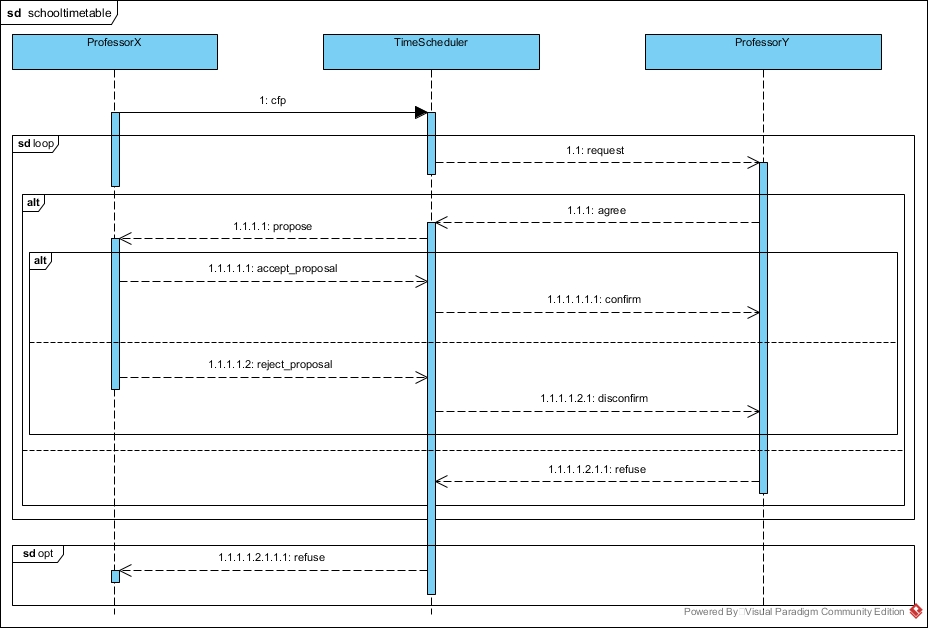
\includegraphics[width=0.60\textwidth]{images/sequence_diagram.jpg}
    \caption{Sequence Diagram of the interaction among agents}
    \label{fig:seq_diagram}
\end{figure}
The interaction among time-scheduler and professors can be explained as follows (as shown in figure \ref{fig:seq_diagram}):\newline
when a professor wants to change an own lesson in order to satisfy a preference, a call-for-proposal (cfp) message is sent to the time-scheduler to begin the negotiation.
The time-scheduler will retrieve the list of all professors who teach in the same class of the proposer's lesson. To have a reasonable change it is also important to consider that for each candidate professor and for each candidate lesson:
\begin{itemize}
    \item the proposer must be free during a candidate lesson
    \item the candidate professor must be free during the lesson the time-scheduler wants to propose.
    \item the proposer's lesson cannot be in the free day of the candidate professor and the candidate lesson cannot be in the free day of the proposer professor
\end{itemize}
Following these criteria, the time-scheduler will realize a list of pair professor-lesson and will try to satisfy the proposer's request with one of them.
The time-scheduler sends to the candidate professor a proposal and this proposal can be accepted according to two criteria:
\begin{itemize}
    \item the proposed lesson is not one of own preferences
    \item the lesson to give must not be in the locked preferences
\end{itemize}
If these criteria are met, the candidate professor replies with an agree message otherwise refuses.
If the reply message contains agree as performative, the time-scheduler communicates to the proposer the possible change. The proposer will accept or reject according to the fact that the lesson change does not worsen own preferences.
According to the last message received from the proposer, the time-scheduler will send to the candidate, who previously accepted the change, a confirm or disconfirm message.
If all possible negotiations fail, the time-scheduler will send to the proposer a refuse message.\newline\newline
\textbf{Ontologies}\newline\newline
As described in \cite{10.1007/3-540-44631-1_7} the content of a message is either a string or a raw sequence of bytes. In realistic case, like in this one, agents need to communicate complex information. When representing complex information, it is necessary to adopt a well-defined syntax so that the content of a message can be parsed by the receiver to extract each specific piece of information. According to FIPA terminology this syntax is known as a content language. FIPA does not mandate a specific content language but defines and recommends the SL language to be used when communicating with the AMS and DF.\newline
For this reason the SL language is used as content language for all messages involving the time-scheduler and the professors. The ontology shared by all agents consists of four concepts and three predicates. The different elements are described with SL syntax as follows:\newline

\textbf{Concepts}
\[(Lesson :hour \langle hour\rangle :day \langle day \rangle)\]
\[(SchoolClass :year \langle year\rangle :letter \langle letter \rangle)\]
\[(Teaching :lesson \langle hour\rangle :schoolClass \langle class \rangle)\]
\[(TimetableConcept :teachings \langle list \: of \: teachings\rangle)\]

\textbf{Predicates}
\[(UpdateTimetable :timetable \langle timetable\:of\:an\:agent \rangle )\]
\[(Change :lessonChange \langle lesson\:related\:to\:a\:change \rangle )\]
\[(Substitution :proposedLesson \langle proposer's \: lesson \rangle :currentLesson \langle candidate's \: lesson \rangle)\]


\textbf{TimetableConcept} is used to encode as content message the timetable of each professor stored as an object of the class \textbf{Timetable}. The reason behind two different classes is due to the fact that \textbf{Timetable} uses a matrix to store information about lessons and it is faster to retrieve and add elements compared to the class \textbf{TimetableConcept}. On the other hand SL language does not support the matrix concept and this is why a concept modelled as a list of teachings is needed.

\subsubsection{Constraint Programming (CP)}\label{subsubsec:case_cp}
In the following part it is provided a mathematical formulation of the model and the corresponding code in Prolog.
The model should be generated dynamically according to the single instance data but to speed up the development process, the current version of this project considers a specific instance of the problem.

\subsubsection{Data provided by the problem}\label{subsubsec:data_problem}
Days of the school week
\[numDays \in \{1..6\} \]
Hours for each school day
\[numHours \in \{1..24\} \]
Number of different professors
\[numProfessors \in \mathbb{N}^+ \]
Number of different classes
\[numClasses \in \mathbb{N}^+ \]
Function which assigns for each professor and each class the number of hours:
\[\forall i \in \{ 1..numProfessors \}\] 
\[ hours_i: \{ 1..numClasses \} \rightarrow \{0..(numHours\:*\:numDays)\} \]
\textbf{Domain of variables}
\[ \forall i \in \{1..numProfessors\}, j \in \{1..numHours\}, k \in \{1..numDays\} \] 
\textbf{PROLOG}
\[P_{ijk} \: in \: 0..numClasses\]
NOTE: 0 is used as joker value to state no class

\subsubsection{Constraints}

\textbf{Each Professor must teach for a specified number of hours in each class}:

\[\forall i \in \{1..numProfessors\}\]
\textbf{PROLOG}
\[ global\_cardinality([P_{i**}],[1-hours_i(1),2-hours_i(2),..,numClass-hours_i(numClass)])\]
NOTE: the number of same values assigned to professor's variables must be equals to the number of hours the professor must spend in that class.

\([P_{i**}]\) means the list of variables associated to professor i
\newline

\textbf{In the same day and hour cannot be more than one professor in each class}

\[\forall j \in \{1..numHours\}, k \in \{1..numDays\}\]
\textbf{PROLOG}
\[all\_distinct\_except\_0([P_{*jk}])\]

NOTE: \([P_{*jk}]\) is the list of variables associated to all professors having the same day and hour.

\textbf{Each Professor must have a free day}
\[\forall i \in \{1..numProfessors\}\]
\textbf{PROLOG}
\[tuples\_in([P_{i*1}],[[0..0]]) \: \lor \: tuples\_in([P_{i*2}],[[0..0]]) \: \lor \: .. \: tuples\_in([P_{i*(numDays)}],[[0..0]])\]

NOTE: \([P_{i*1}]\) is the list of all variables of professor i at day 1 for all hours.

\subsubsection{Performance}

The solution of the CP model requires a lot of time to be computed because of the huge amount of variables and constraints imposed on them. Therefore a \textbf{DummyBehaviour} has been realized to simulate the creation of the professors' timetable and then each timetable is sent to the corresponding professor.